% !TEX root = ../../Main.tex
\section{Trading Framework: The Environment the Agent Trades In}
\label{Section:TradingFramework}

No existing framework could both train an agent offline on quote-level history and run the same agent on a live account without rewriting it. Building one took a large part of the effort in this work. Its design choices decide how far the results in \Cref{Chapter:ExperimentalResults} can be trusted. Three properties were required. First, the tested system and the deployed system had to be the same code, so that a result obtained offline says something about live behaviour. Second, the data had to have a fine enough resolution to rebuild the price path inside a bar, because that path decides what a position actually paid. Third, the costs had to be the costs of a real account, not simplified values chosen for convenience.

\subsection{System Architecture: Three Execution Contexts}

The framework has to be written in two languages. The strategy logic, the learning models and the market abstractions are written in Python, which has the numerical and machine learning libraries. Access to the broker is written in C\#, because cTrader \cite{noauthor_forex_nodate} runs algorithmic strategies as cBots on the .NET runtime and offers no other way to reach its order book. The two parts communicate through named memory-mapped files with paired auto-reset event handles, one pair for each direction. They work as a single-slot request and response exchange. The platform writes an update and signals. Python reads it, writes an action and signals back, and then the platform continues. Two kinds of message cross this boundary. Updates go from the platform to Python, and actions go the other way. \Cref{Figure:SystemArchitecture} shows the arrangement. The important result of this design is that the strategy object does not know where its updates come from. The same class, with the same weights, runs in three contexts.

\begin{figure}[htb!]
\centering
\begin{tikzpicture}[
  node distance=6mm,
  box/.style={draw, rounded corners=2pt, align=center, font=\small, minimum height=8mm, inner sep=3pt},
  wide/.style={box, text width=34mm},
  narrow/.style={box, text width=26mm},
  lbl/.style={font=\scriptsize\itshape},
  flow/.style={-stealth, thick},
  dashflow/.style={-stealth, thick, dashed}
]
\node[wide] (broker) {Broker\\\scriptsize IC Markets, raw spread, swap-free};
\node[wide, below=of broker] (platform) {cTrader platform};
\node[wide, below=of platform] (cbot) {Connector cBot\\\scriptsize C\# / .NET};
\node[narrow, right=14mm of cbot] (bridge) {Shared memory\\\scriptsize updates $\rightarrow$\\\scriptsize $\leftarrow$ actions};
\node[wide, right=14mm of bridge] (library) {Python library};
\node[narrow, above=8mm of library] (market) {Market abstractions\\\scriptsize ticks, bars, indicators};
\node[narrow, above=8mm of market] (strategy) {Strategy\\\scriptsize DDPG agent};
\node[narrow, below=8mm of library] (portfolio) {Portfolio\\\scriptsize orders, positions, costs};
\node[wide, below=14mm of cbot] (database) {Market database\\\scriptsize PostgreSQL, quote level};

\draw[flow] (broker) -- (platform);
\draw[flow] (platform) -- (cbot);
\draw[flow] (cbot) -- (bridge);
\draw[flow] (bridge) -- (library);
\draw[flow] (library) -- (market);
\draw[flow] (market) -- (strategy);
\draw[flow] (library) -- (portfolio);
\draw[flow] (platform.east) to[out=0, in=90] (bridge.north);
\draw[dashflow] (database) -| (library);
\node[lbl, below=1mm of database] {offline replay bypasses the platform};
\end{tikzpicture}
\caption{Framework architecture. The strategy receives updates and returns actions. It does not know whether the updates come from a live account, from the platform's own backtester or from the stored quote database.}
\label{Figure:SystemArchitecture}
\end{figure}

In the first context the platform is not used. Python replays stored quotes directly from the market database. This is the fastest of the three contexts, and it is the one used for training and for every result reported in this work. In the second context the strategy runs inside cTrader's own backtesting tab on the platform's historical data. This gives an independent check of the offline engine. In the third context the same strategy runs on a live account. It receives real quotes and sends real orders. The benefit of this design is that the three contexts differ only in where the updates come from. When a strategy behaves one way in a backtest and another way when deployed, the usual cause is two separate implementations that have diverged over time. Here there is only one implementation, so this problem does not occur.

\subsection{Market Data: Collection, Storage and Resolution}

The historical data was collected through the same connector. The C\# component requested it from cTrader, and the Python component wrote it to a local PostgreSQL database. Two types of record are stored. A tick holds the bid and ask quoted at one instant, together with the conversion rates needed to express a profit or loss in the account currency at that instant. A bar holds its open, high, low and close as references to the ticks that produced them. A bar is therefore a view of the tick tape, not a separate copy of the prices. \Cref{Tables:DataInventory} lists the data held for the seven pairs. The tick tape is the primary record, and the bar series are derived from it. This is what allows the engine to rebuild the path a price took inside a bar, instead of interpolating between its end points.

% !TEX root = ../Main.tex
\begin{table}[htb!]
\centering
\footnotesize
\caption{Market data collected from cTrader and stored locally, from January 2014 to August 2026. The tick tape takes 295 GB and is the primary record. The bar series point to the ticks that produced them.}
\label{Tables:DataInventory}
\begin{tabular}{@{}lrrrrr@{}}
\toprule
\textbf{Pair} & \textbf{Ticks} & \textbf{M1 bars} & \textbf{H1 bars} & \textbf{D1 bars} & \textbf{MN1 bars} \\
\midrule
AUD/USD & 227,914,614 & 4,643,990 & 78,320 & 3,346 & 150 \\
EUR/USD & 242,847,954 & 4,636,138 & 78,145 & 3,339 & 150 \\
GBP/USD & 281,490,557 & 4,648,216 & 78,311 & 3,339 & 150 \\
NZD/USD & 203,788,307 & 4,631,614 & 78,282 & 3,339 & 150 \\
USD/CAD & 228,356,007 & 4,635,179 & 78,319 & 3,347 & 150 \\
USD/CHF & 194,186,979 & 4,621,503 & 78,307 & 3,338 & 150 \\
USD/JPY & 284,430,458 & 4,638,775 & 78,151 & 3,338 & 150 \\
\midrule
\textbf{Total} & \textbf{1,663,014,876} & \textbf{32,455,415} & \textbf{547,835} & \textbf{23,386} & \textbf{1,050} \\
\bottomrule
\end{tabular}
\end{table}

Two properties of this data must be stated, because otherwise both would look like defects.

Bars are stamped at the close of the broker's trading session, not at midnight. This is at 22:00 UTC, or at 21:00 under daylight saving. A daily series therefore has five bars in a normal week, stamped Sunday to Thursday, and the bar stamped Thursday holds Friday's session. An audit against a calendar-day reference reports every Friday as missing. This is a result of the stamping convention, and no data is lost. The period from 11 to 25 January 2016 is missing from all seven pairs, both in ticks and in bars. The gap comes from the broker. A new download of those days returned nothing, which confirmed that the gap cannot be repaired. The gap is the same for all seven pairs, so it does not bias any comparison between them. It also falls outside the evaluation window used in \Cref{Chapter:ExperimentalResults}.

\subsection{Cost Model: Spread, Commission and Account Type}

The execution engine advances on ticks, not on bar closes. A position opened during a bar is filled at a quote that existed within that bar. A stop or target attached to it is tested against the quotes in the order they arrived. This matters for the reason given in \Cref{Chapter:RelatedWork}. A bar reports four prices but hides the order in which the price reached them. That order decides whether a stop was reached before a target, and which spread was crossed.

The account modelled is a swap-free raw-spread retail account. Each of the three charges described in \Cref{Section:PerformanceMeasurement} is applied at the rate that such an account pays. A buy is filled at the ask and a sell at the bid, both read from the tick tape at the instant of the fill. The spread is therefore charged by construction, as part of every fill, and is not deducted afterwards. The commission is charged on traded volume at $3.5$ points per side. For a standard lot of $100{,}000$ units this is $3.5$ units of the quote currency per side, or $7$ per round turn. The swap is zero. On a swap-free account this is the rate the account really charges, so it is not an approximation. \Cref{Tables:CostModel} lists the full configuration.

% !TEX root = ../Main.tex
\begin{table}[htb!]
\centering
\footnotesize
\caption{Cost and account configuration applied to every evaluation reported in this work.}
\label{Tables:CostModel}
\begin{tabularx}{\textwidth}{@{}llX@{}}
\toprule
\textbf{Setting} & \textbf{Value} & \textbf{Meaning} \\
\midrule
Account type & Raw spread, swap-free & An account that a retail client can open, with the interbank spread and no charge for overnight financing \\
\addlinespace
Spread & Accurate & The bid-ask difference recorded at the moment of the trade, read from the tick tape and not assumed \\
\addlinespace
Commission & 3.5 points per side & Charged on traded volume. This is 3.5 units of the quote currency per standard lot per side, or 7 per round turn \\
\addlinespace
Swap & 0 points & The rate a swap-free account charges, so not an approximation \\
\addlinespace
Account currency & EUR & Profit and loss converted at the rate recorded on the tick that produced it \\
\addlinespace
Initial balance & 10,000 & Reported across five starting balances, as described in \Cref{Chapter:ExperimentalResults} \\
\addlinespace
Leverage & 30 & The retail limit for major currency pairs \\
\addlinespace
Position mode & Netting & One net position per instrument, not separate hedged positions \\
\bottomrule
\end{tabularx}
\end{table}

The choice to read the spread from the ticks, instead of assuming a value for it, should be supported with data. Assuming a value is common, and the error it causes is not small. \Cref{Figure:SpreadOverTime} plots the monthly mean spread of each pair across the evaluation window. For EUR/USD, the most liquid pair in the market, the monthly mean goes from $0.77$ to $13.00$ points. This is a factor of seventeen between the quietest month and the busiest one. USD/CHF reaches $37.82$ points in January 2015, when the Swiss National Bank removed its floor against the Euro. For each of the seven pairs, the spread in the widest month is at least five times the spread in the narrowest month.

\begin{figure}[htb!]
\centering
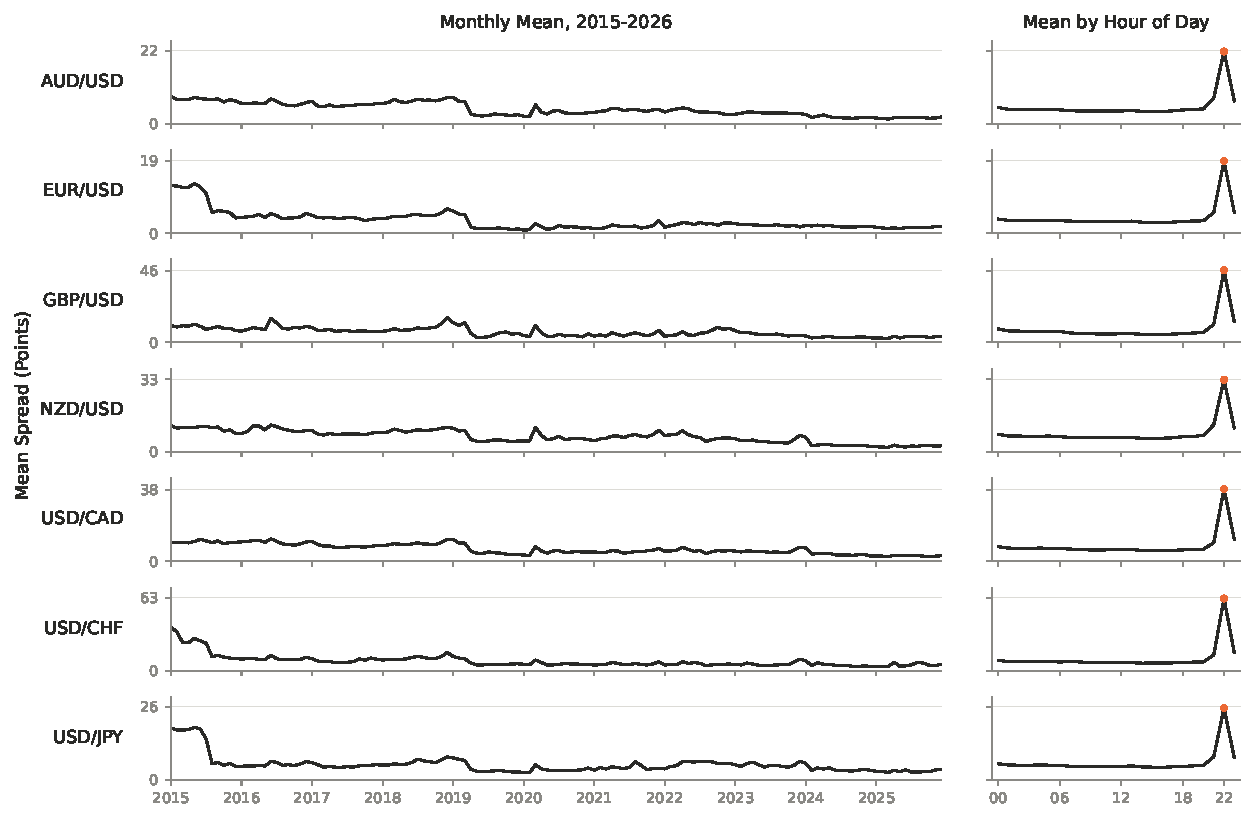
\includegraphics[width=\textwidth]{Images/SpreadOverTime.pdf}
\caption{Monthly mean spread in points for the seven major pairs, 2015 to 2026, computed from the full tick tape. EUR/USD is drawn in black. A model evaluated at a fixed spread is evaluated in market conditions that do not occur in any month of this sample.}
\label{Figure:SpreadOverTime}
\end{figure}

The pattern of this variation matters more than its size. Spreads widen when liquidity falls and around the events that move prices. These are the moments when a model trained on an average spread is most likely to act. A strategy charged a constant spread is therefore charged the wrong amount, and the error is correlated with its own trading activity. The error also goes in the direction that makes the strategy look better.

The engine was validated against cTrader's own backtester, not against itself. Six reference configurations were used, covering two currency pairs and three windows. In all of them, the engine's trade, position, order and deal records reproduce the platform's output byte for byte. The conversion of profit and loss into the account currency was also checked separately against the platform's own figures. The only divergence is sub-pip. It comes from the resolution of the stored quotes, not from the accounting. The engine therefore reproduces the platform it was built against, and it can also do more than that platform. The same strategy is evaluated offline directly on the tick tape. This runs at a speed that the platform's own backtester cannot reach, and over windows that the backtester will not cover. The cost model can be set to any account the broker offers, not only to the account the terminal happens to be connected to.

Two consequences follow. Both are stated here so that \Cref{Chapter:ExperimentalResults} can be read correctly. First, the returns reported in this work are net of the spread actually quoted and of a real commission schedule. They are therefore lower than the same policy would show on bar closes with a fixed spread or no spread, and they cannot be compared directly with results obtained in that way. Second, because the account is swap-free, no financing cost is estimated or left out. A strategy that holds positions over many nights is charged exactly what such an account would charge it.